\documentclass{article}

\usepackage[utf8]{inputenc}
\usepackage[top=3cm, headheight=2.2cm, headsep=10pt]{geometry}
\usepackage{graphicx}

% To reference the last page
\usepackage{lastpage}

% Like `tabularx` but supports pagebreaks
\usepackage{ltablex}
% Adjust row vertical spacing
\renewcommand{\arraystretch}{1.2}

% Multiline cells
\usepackage{makecell}

% Set date format to ISO 8601
\usepackage{datetime}
\newdateformat{isodate}{\THEYEAR-\twodigit{\THEMONTH}-\twodigit{\THEDAY}}

% Table colouring
\usepackage[table,dvipsnames]{xcolor}
\definecolor{tableHeaderColor}
{rgb}{0.75,0.75,0.75}
\definecolor{tableColumnColor}
{rgb}{0.95, 0.95, 0.95}
\definecolor{notesColor}
{rgb}{0.95, 0.95, 0.95}
\definecolor{highlightColor}
{rgb}{1.00, 0.95, 0.80}

% Icons for checkbox
\usepackage{pifont}

% Command to create a checkbox
\newcommand{\checkbox}{\ding{113}}

% For automatic counters
\usepackage{array}

% Header and footer
\usepackage{fancyhdr}
\pagestyle{fancy}
\fancyhf{} % Clear header and footer
\renewcommand{\headrulewidth}{0pt}
\lhead{\includegraphics[width=2cm]{../../common/assets/HELIOS_LOGO.png}}
\rhead{\includegraphics[width=2cm]{../../common/assets/ARIS_space_to_grow_LOGO-black.pdf}}
\cfoot{\thepage}
\fancyfoot[L]{Project HEPHAESTUS}
\fancyfoot[C]{Page \thepage\ out of \pageref{LastPage}}

% Draft watermark
\newboolean{isDraft}
\setboolean{isDraft}{true} % Set to false to remove the watermark
\ifthenelse{\boolean{isDraft}}{
  \usepackage{background}
  \backgroundsetup{
    scale=25,
    color=gray,
    opacity=0.4,
    angle=45,
    position=current page.center,
    contents={Draft}
  }
}{}

% Highlight colour
\usepackage{soul}
\sethlcolor{magenta}

% Strikethrough
\usepackage[normalem]{ulem}

% Clickable Hyperlinks
\usepackage[colorlinks=true, linkcolor=blue, urlcolor=blue]{hyperref}

% Toggleable procedure items
\usepackage{etoolbox}



% Command for row in note list
\newcommand{\noteItem}[1]{
  \begin{minipage}[t]{\linewidth}
    #1
    \vspace{1mm} % Just slightly add vspace to prevent clipping into table border
  \end{minipage}
  \\ \hline
}

\title{Contingency Procedures Master}
\author{Guideline}
\date{Version: \isodate\today}

\begin{document}

\maketitle

% Set the page style for the title page
\thispagestyle{fancy}

\section{Operation Phases}

\begin{tabularx}{0.9\textwidth}{|X|X|}
  \hline
  \begin{minipage}[t]{\linewidth} \textbf{Current Phase} \\ (mark with magnet) \vspace{1mm} \end{minipage} & \textbf{System State}  \\ \hline
  \begin{minipage}[t]{\linewidth} 3 Preparation \& Assembly \\ 4 Transfer to Airfield \\ 5 Installation \& Pre-Firing Checks \\ 9 Post-Firing Checks \& Deinstallation \\ 10 Return to IPZ \\ 11 Disassembly \& Inspection \vspace{1mm} \end{minipage} & \cellcolor{green} System is safe \\ \hline
  \begin{minipage}[t]{\linewidth} 6 Filling \& Ignition Test \\ 8 Safe State Establishment \vspace{1mm} \end{minipage} & \cellcolor{red} System is pressurized \\ \hline
  \begin{minipage}[t]{\linewidth}
    7 Firing
    \vspace{1mm}
  \end{minipage}
  & \cellcolor{red} Firing: HUT closed \\ \hline
\end{tabularx}

\section{Contingency Procedures}
\begin{tabularx}{0.9\textwidth}{|X|}
    \cellcolor{blue} \textcolor{white}{General} \\ \hline
    HEP\_CP\_GEN\_001\_Injury\_XX \\ \hline
    HEP\_CP\_GEN\_002\_Fire\_XX \\ \hline
    HEP\_CP\_GEN\_003\_Trespassing\_XX \\ \hline
    \cellcolor{orange} PSS \\ \hline
    HEP\_CP\_PSS\_004\_Leakage\_XX \\ \hline
    HEP\_CP\_PSS\_005\_Overpressure\_XX \\ \hline
    HEP\_CP\_PSS\_006\_BottleValve-Anomaly\_XX \\ \hline
    HEP\_CP\_PSS\_007\_NoisesHissing\_XX \\ \hline
    \cellcolor{yellow} DACS \\ \hline
    HEP\_CP\_DACS\_001\_PowerLoss\_XX \\ \hline
    HEP\_CP\_DACS\_002\_ConnectionLoss\_XX \\ \hline
    HEP\_CP\_DACS\_003\_ValveAnomalies\_XX \\ \hline
\end{tabularx}
\newpage
\section{Telephone Protocol}
\begin{itemize}
    \item Where? Address of the HUT:
    \begin{itemize}
        \item Flughafen Dübendorf – Hunter Stübli (HUT)
        \item Rechweg
        \item 8600 Dübendorf
    \end{itemize}
    \item Who? (your name and how you can be contacted)
    \item What happended?
    \item When did it happen?
    \item How many injured? What injuries?
    \item Additional Information?
    \item Wait for Questions; do not hang up!
\end{itemize}

\section{Location Plan}
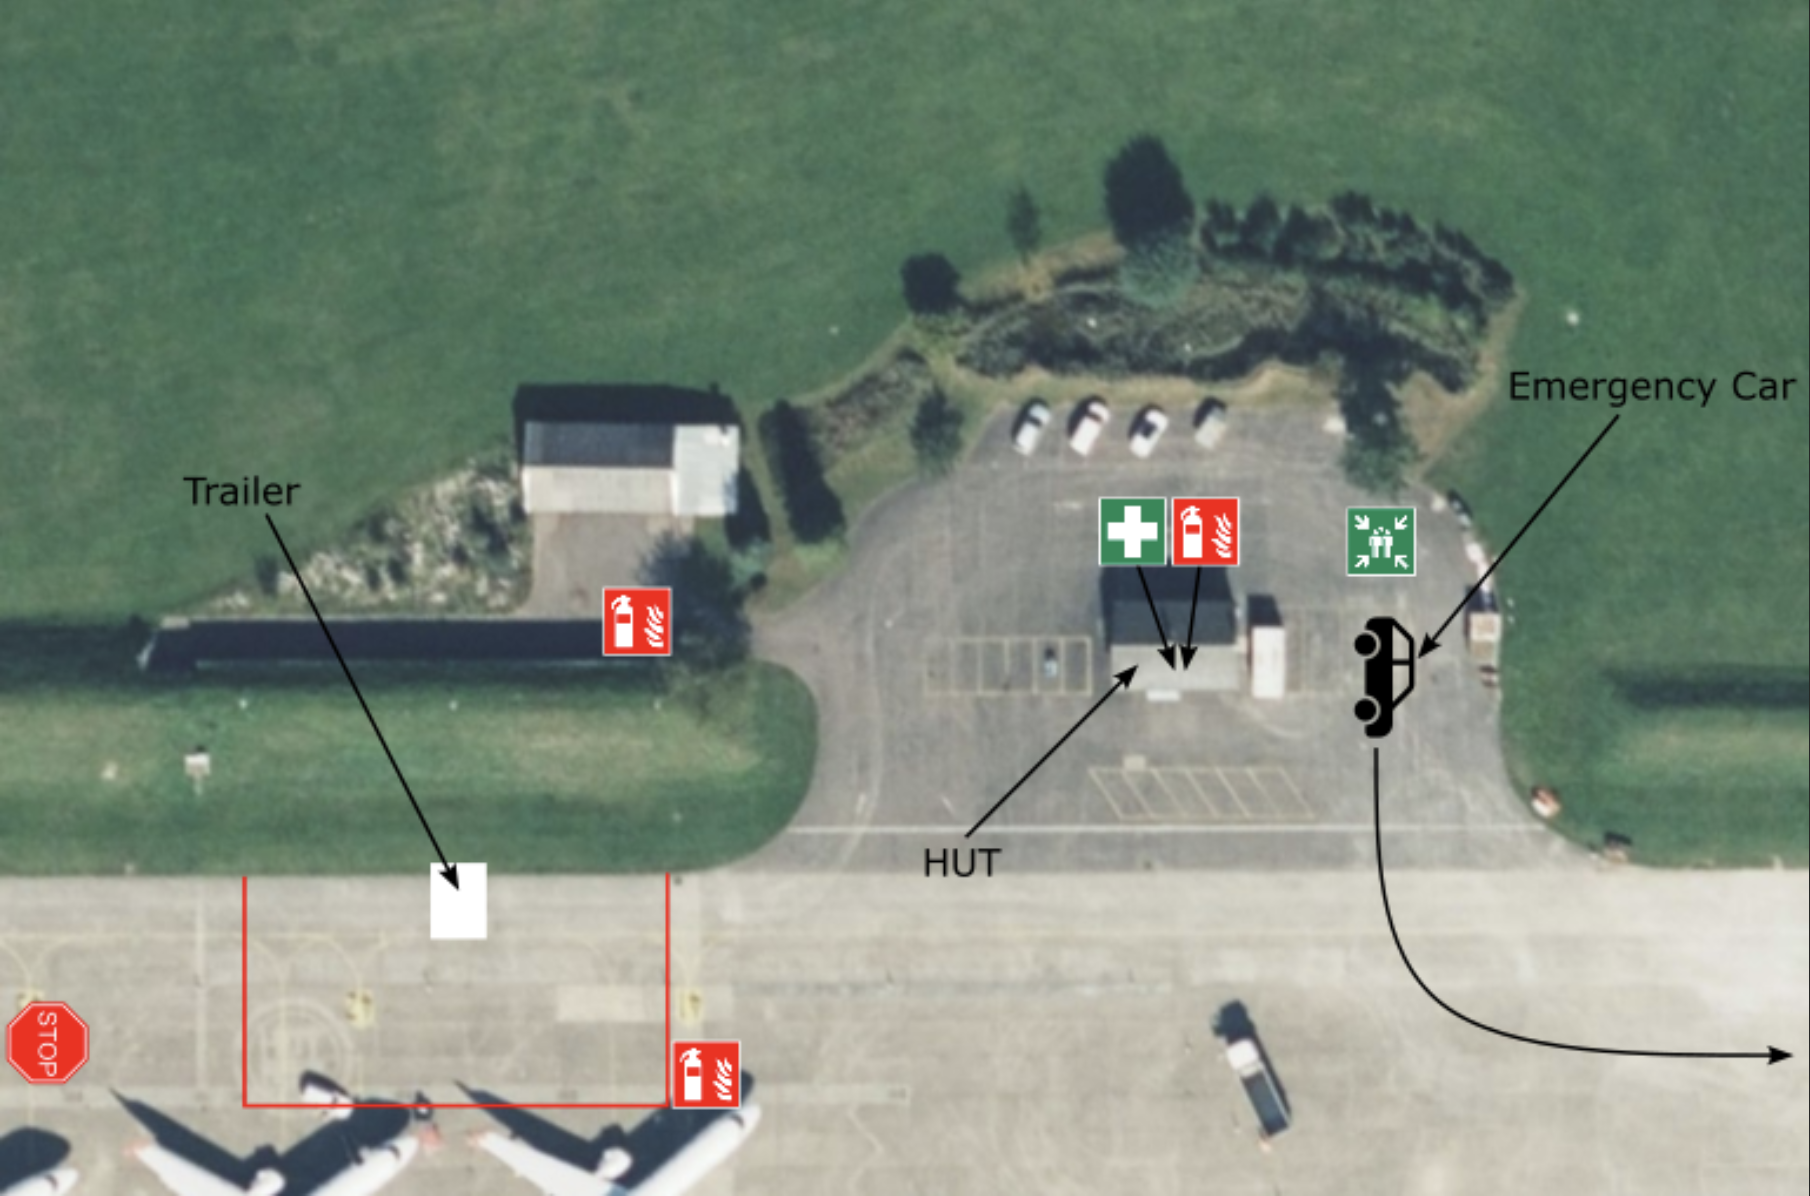
\includegraphics[width=\textwidth]{assets/location_map.png}
\newpage
\section{Emergency Numbers}
\begin{tabularx}{0.9\textwidth}{|>{\columncolor{tableColumnColor}}c|X|}
    \hline
    Ambulance & 144 \\ \hline
    Rega & 1414 \\ \hline
    Fire service & 118 \\ \hline
    Police & 117 \\ \hline
    Toxics & 145 \\ \hline
\end{tabularx}

\begin{tabularx}{0.9\textwidth}{|>{\columncolor{tableColumnColor}}c|X|X|}
    \hline
    \rowcolor{tableHeaderColor} Entity & Adress & Phone Number \\ \hline
    HUT & \begin{minipage}{\linewidth}
        \vspace{1mm}
        Flughafen Dübendorf HUT \\
        Rechweg \\
        8600 Dübendorf
        \vspace{1mm}
    \end{minipage} & - \\ \hline
    Spital Uster & \begin{minipage}{\linewidth}
        \vspace{1mm}
        Brunnenstrasse 42 \\
        8610 Uster
        \vspace{1mm}
    \end{minipage} & +41 44 911 11 11 \\ \hline
    Airfield Responsible & Roger Gisler & \begin{minipage}{\linewidth}
        \vspace{1mm}
        +41 58 481 79 18 \\
        If not reachable: \\
        +41 79 944 42 52
        \vspace{1mm}
    \end{minipage} \\ \hline
    President ARIS & Chloé Pilloud & +41 79 226 39 42 \\ \hline
    HEPHAESTUS Supervisor & Philip Wolf & +41 79 386 01 28 \\ \hline
\end{tabularx}

\section{Emergency Responsibilities}

\begin{tabularx}{0.9\textwidth}{|>{\columncolor{tableColumnColor}}c|X|}
    \hline
    \rowcolor{tableHeaderColor} Responsibility & Name \\ \hline
    Emergency Driver 1 & \underline{\hspace{5cm}} \\ \hline
    Emergency Driver 2 & \underline{\hspace{5cm}} \\ \hline
    Emergency Helper 1 & \underline{\hspace{5cm}} \\ \hline
    Emergency Helper 2 & \underline{\hspace{5cm}} \\ \hline
\end{tabularx}
\newpage
\section{Manual Override Box States}
\begin{tabularx}{0.9\textwidth}{|>{\columncolor{tableColumnColor}}X|X|X|}
    \hline
    \rowcolor{tableHeaderColor} \multicolumn{3}{|c|}{\large{NO CIRCUIT ARMED}} \\ \hline
    \rowcolor{tableHeaderColor} Subpart & State & Controllable? \\ \hline
    Main Valve (OSS MAIN) & CLOSED & \cellcolor{red} NO \\ \hline
    Main Valve (FSS MAIN) & CLOSED & \cellcolor{red} NO \\ \hline
    Control Valve (OSS MAIN) & OPEN & \cellcolor{red} NO \\ \hline
    Control Valve (FSS MAIN) & OPEN & \cellcolor{red} NO \\ \hline
    Vent Valve (OSS) & OPEN & \cellcolor{red} NO \\ \hline
    Vent Valve (FSS) & OPEN & \cellcolor{red} NO \\ \hline
    Fill Valve (OSS) & CLOSED & \cellcolor{red} NO \\ \hline
    Drain Valve (FSS) & CLOSED & \cellcolor{red} NO \\ \hline
    Pressurization Valve (OSS PRZ) & CLOSED & \cellcolor{red} NO \\ \hline
    Pressurization Valve (FSS PRZ) & CLOSED & \cellcolor{red} NO \\ \hline
    Main Valve (H2 IGN) & CLOSED & \cellcolor{red} NO \\ \hline
    Main Valve (O2 MAIN) & CLOSED & \cellcolor{red} NO \\ \hline
    Purge Valve (OSS) & CLOSED & \cellcolor{red} NO \\ \hline
    Purge Valve (FSS) & CLOSED & \cellcolor{red} NO \\ \hline
    Purge Valve (IGN) & CLOSED & \cellcolor{red} NO \\ \hline
    Spark Plug & OFF & \cellcolor{red} NO \\ \hline
\end{tabularx}
\newpage
\begin{tabularx}{0.9\textwidth}{|>{\columncolor{tableColumnColor}}X|X|X|}
    \hline
    \rowcolor{tableHeaderColor} \multicolumn{3}{|c|}{\large{MANUAL ABORT}} \\ \hline
    \rowcolor{tableHeaderColor} Subpart & State & Controllable? \\ \hline
    Main Valve (OSS MAIN) & CLOSED & \cellcolor{red} NO \\ \hline
    Main Valve (FSS MAIN) & CLOSED & \cellcolor{red} NO \\ \hline
    Control Valve (OSS MAIN) & OPEN & \cellcolor{red} NO \\ \hline
    Control Valve (FSS MAIN) & OPEN & \cellcolor{red} NO \\ \hline
    Vent Valve (OSS) & OPEN & \cellcolor{red} NO \\ \hline
    Vent Valve (FSS) & OPEN & \cellcolor{red} NO \\ \hline
    Fill Valve (OSS) & CLOSED & \cellcolor{red} NO \\ \hline
    Drain Valve (FSS) & CLOSED & \cellcolor{red} NO \\ \hline
    Pressurization Valve (OSS PRZ) & CLOSED & \cellcolor{red} NO \\ \hline
    Pressurization Valve (FSS PRZ) & CLOSED & \cellcolor{red} NO \\ \hline
    Main Valve (H2 IGN) & CLOSED & \cellcolor{red} NO \\ \hline
    Main Valve (O2 MAIN) & CLOSED & \cellcolor{red} NO \\ \hline
    Purge Valve (OSS) & CLOSED & \cellcolor{red} NO \\ \hline
    Purge Valve (FSS) & CLOSED & \cellcolor{red} NO \\ \hline
    Purge Valve (IGN) & CLOSED & \cellcolor{red} NO \\ \hline
    Spark Plug & OFF & \cellcolor{red} NO \\ \hline
\end{tabularx}
\newpage
\begin{tabularx}{0.9\textwidth}{|>{\columncolor{tableColumnColor}}X|X|X|}
    \hline
    \rowcolor{tableHeaderColor} \multicolumn{3}{|c|}{\large{FSS FILL ARMED}} \\ \hline
    \rowcolor{tableHeaderColor} Subpart & State & Controllable? \\ \hline
    Main Valve (OSS MAIN) & CLOSED & \cellcolor{red} NO \\ \hline
    Main Valve (FSS MAIN) & CLOSED & \cellcolor{red} NO \\ \hline
    Control Valve (OSS MAIN) & OPEN & \cellcolor{red} NO \\ \hline
    Control Valve (FSS MAIN) & OPEN & \cellcolor{red} NO \\ \hline
    Vent Valve (OSS) & OPEN or CLOSED& \cellcolor{green} YES \\ \hline
    Vent Valve (FSS) & OPEN or CLOSED & \cellcolor{green} YES \\ \hline
    Fill Valve (OSS) & CLOSED & \cellcolor{red} NO \\ \hline
    Drain Valve (FSS) & CLOSED or OPEN & \cellcolor{green} YES \\ \hline
    Pressurization Valve (OSS PRZ) & CLOSED & \cellcolor{red} NO \\ \hline
    Pressurization Valve (FSS PRZ) & CLOSED & \cellcolor{red} NO \\ \hline
    Main Valve (H2 IGN) & CLOSED & \cellcolor{red} NO \\ \hline
    Main Valve (O2 MAIN) & CLOSED & \cellcolor{red} NO \\ \hline
    Purge Valve (OSS) & CLOSED or OPEN & \cellcolor{green} YES \\ \hline
    Purge Valve (FSS) & CLOSED or OPEN & \cellcolor{green} YES \\ \hline
    Purge Valve (IGN) & CLOSED or OPEN & \cellcolor{green} YES \\ \hline
    Spark Plug & OFF & \cellcolor{red} NO \\ \hline
\end{tabularx}
\newpage
\begin{tabularx}{0.9\textwidth}{|>{\columncolor{tableColumnColor}}X|X|X|}
    \hline
    \rowcolor{tableHeaderColor} \multicolumn{3}{|c|}{\large{OSS PRE-FILL ARMED}} \\ \hline
    \rowcolor{tableHeaderColor} Subpart & State & Controllable? \\ \hline
    Main Valve (OSS MAIN) & CLOSED or OPEN& \cellcolor{green} YES \\ \hline
    Main Valve (FSS MAIN) & CLOSED & \cellcolor{red} NO \\ \hline
    Control Valve (OSS MAIN) & OPEN & \cellcolor{red} NO \\ \hline
    Control Valve (FSS MAIN) & OPEN & \cellcolor{red} NO \\ \hline
    Vent Valve (OSS) & OPEN or CLOSED& \cellcolor{green} YES \\ \hline
    Vent Valve (FSS) & OPEN or CLOSED& \cellcolor{green} YES \\ \hline
    Fill Valve (OSS) & CLOSED or OPEN& \cellcolor{green} YES \\ \hline
    Drain Valve (FSS) & CLOSED & \cellcolor{red} NO \\ \hline
    Pressurization Valve (OSS PRZ) & CLOSED or OPEN & \cellcolor{green} YES \\ \hline
    Pressurization Valve (FSS PRZ) & CLOSED & \cellcolor{red} NO \\ \hline
    Main Valve (H2 IGN) & CLOSED & \cellcolor{red} NO \\ \hline
    Main Valve (O2 MAIN) & CLOSED & \cellcolor{red} NO \\ \hline
    Purge Valve (OSS) & CLOSED or OPEN &  \cellcolor{green} YES \\ \hline
    Purge Valve (FSS) & CLOSED or OPEN &  \cellcolor{green} YES \\ \hline
    Purge Valve (IGN) & CLOSED or OPEN &  \cellcolor{green} YES \\ \hline
    Spark Plug & OFF & \cellcolor{red} NO \\ \hline
\end{tabularx}
\newpage
\begin{tabularx}{0.9\textwidth}{|>{\columncolor{tableColumnColor}}X|X|X|}
    \hline
    \rowcolor{tableHeaderColor} \multicolumn{3}{|c|}{\large{OSS FILL ARMED}} \\ \hline
    \rowcolor{tableHeaderColor} Subpart & State & Controllable? \\ \hline
    Main Valve (OSS MAIN) & CLOSED & \cellcolor{red} NO \\ \hline
    Main Valve (FSS MAIN) & CLOSED & \cellcolor{red} NO \\ \hline
    Control Valve (OSS MAIN) & OPEN & \cellcolor{red} NO \\ \hline
    Control Valve (FSS MAIN) & OPEN & \cellcolor{red} NO \\ \hline
    Vent Valve (OSS) & OPEN or CLOSED & \cellcolor{green} YES \\ \hline
    Vent Valve (FSS) & OPEN or CLOSED & \cellcolor{green} YES \\ \hline
    Fill Valve (OSS) & CLOSED or OPEN& \cellcolor{green} YES \\ \hline
    Drain Valve (FSS) & CLOSED & \cellcolor{red} NO \\ \hline
    Pressurization Valve (OSS PRZ) & CLOSED & \cellcolor{red} NO \\ \hline
    Pressurization Valve (FSS PRZ) & CLOSED & \cellcolor{red} NO \\ \hline
    Main Valve (H2 IGN) & CLOSED & \cellcolor{red} NO \\ \hline
    Main Valve (O2 MAIN) & CLOSED & \cellcolor{red} NO \\ \hline
    Purge Valve (OSS) & CLOSED or OPEN & \cellcolor{green} YES \\ \hline
    Purge Valve (FSS) & CLOSED or OPEN & \cellcolor{green} YES \\ \hline
    Purge Valve (IGN) & CLOSED or OPEN & \cellcolor{green} YES \\ \hline
    Spark Plug & OFF & \cellcolor{red} NO \\ \hline
\end{tabularx}
\newpage
\begin{tabularx}{0.9\textwidth}{|>{\columncolor{tableColumnColor}}X|X|X|}
    \hline
    \rowcolor{tableHeaderColor} \multicolumn{3}{|c|}{\large{FIRING ARMED}} \\ \hline
    \rowcolor{tableHeaderColor} Subpart & State & Controllable? \\ \hline
    Main Valve (OSS MAIN) & OPEN or CLOSED & \cellcolor{green} YES \\ \hline
    Main Valve (FSS MAIN) & OPEN or CLOSED & \cellcolor{green} YES \\ \hline
    Control Valve (OSS MAIN) & OPEN or CLOSED & \cellcolor{green} YES \\ \hline
    Control Valve (FSS MAIN) & OPEN or CLOSED & \cellcolor{green} YES \\ \hline
    Vent Valve (OSS) & OPEN or CLOSED & \cellcolor{green} YES \\ \hline
    Vent Valve (FSS) & OPEN or CLOSED & \cellcolor{green} YES \\ \hline
    Fill Valve (OSS) & CLOSED & \cellcolor{red} NO \\ \hline
    Drain Valve (FSS) & OPEN or CLOSED & \cellcolor{green} YES \\ \hline
    Pressurization Valve (OSS PRZ) & OPEN or CLOSED & \cellcolor{green} YES \\ \hline
    Pressurization Valve (FSS PRZ) & OPEN or CLOSED & \cellcolor{green} YES \\ \hline
    Main Valve (H2 IGN) & OPEN or CLOSED & \cellcolor{green} YES \\ \hline
    Main Valve (O2 MAIN) & OPEN or CLOSED & \cellcolor{green} YES \\ \hline
    Purge Valve (OSS) & OPEN or CLOSED & \cellcolor{green} YES \\ \hline
    Purge Valve (FSS) & OPEN or CLOSED & \cellcolor{green} YES \\ \hline
    Purge Valve (IGN) & OPEN or CLOSED & \cellcolor{green} YES \\ \hline
    Spark Plug & OFF & \cellcolor{red} NO \\ \hline
\end{tabularx}
\newpage
\begin{tabularx}{0.9\textwidth}{|>{\columncolor{tableColumnColor}}X|X|X|}
    \hline
    \rowcolor{tableHeaderColor} \multicolumn{3}{|c|}{\large{IGNITION KEY TURNED}} \\ \hline
    \rowcolor{tableHeaderColor} Subpart & State & Controllable? \\ \hline
    Main Valve (OSS MAIN) & CLOSED & \cellcolor{red} NO \\ \hline
    Main Valve (FSS MAIN) & CLOSED & \cellcolor{red} NO \\ \hline
    Control Valve (OSS MAIN) & OPEN & \cellcolor{red} NO \\ \hline
    Control Valve (FSS MAIN) & OPEN & \cellcolor{red} NO \\ \hline
    Vent Valve (OSS) & OPEN & \cellcolor{red} NO \\ \hline
    Vent Valve (FSS) & OPEN & \cellcolor{red} NO \\ \hline
    Fill Valve (OSS) & CLOSED & \cellcolor{red} NO \\ \hline
    Drain Valve (FSS) & CLOSED & \cellcolor{red} NO \\ \hline
    Pressurization Valve (OSS PRZ) & CLOSED & \cellcolor{red} NO \\ \hline
    Pressurization Valve (FSS PRZ) & CLOSED & \cellcolor{red} NO \\ \hline
    Main Valve (H2 IGN) & CLOSED & \cellcolor{red} NO \\ \hline
    Main Valve (O2 MAIN) & CLOSED & \cellcolor{red} NO \\ \hline
    Purge Valve (OSS) & CLOSED & \cellcolor{red} NO \\ \hline
    Purge Valve (FSS) & CLOSED & \cellcolor{red} NO \\ \hline
    Purge Valve (IGN) & CLOSED & \cellcolor{red} NO \\ \
    Spark Plug & OFF or ON & \cellcolor{green} YES \\ \hline
\end{tabularx}
\newpage
\section{Notes}
% Notes

\rowcolors{1}{notesColor}{notesColor}
\begin{tabularx}{\textwidth}{X}
  \hline

  \noteItem{}
  \noteItem{}
  \noteItem{}
  \noteItem{}
  \noteItem{}
  \noteItem{}
  \noteItem{}
  \noteItem{}
  \noteItem{}
  \noteItem{}
  \noteItem{}
  \noteItem{}
  \noteItem{}
  \noteItem{}
  \noteItem{}
  \noteItem{}
  \noteItem{}
  \noteItem{}
  \noteItem{}
  \noteItem{}
  \noteItem{}
  \noteItem{.}
  
\end{tabularx}

\end{document}